\section{Examples}
\label{sec:examples}
In order to demonstrate our work, we show the creation of a variety of visualization using VisComposer.  Examples range from network and hierarchical datasets to structured and unstructured data. In each example explained below, the flexibility of VisComposer is highlighted. Please view the supplementary video for more details.

\subsection{Scatterplot Matrix}
 % pure interaction
Typically, a scatterplot matrix consists of neatly arranged scatterplots, each of which represents two of the dimensions. Because each of the diagonal cells has the same dimension bound to the \emph{x} and \emph{y} coordinates, the resultant visualization of those individual scatterplots will always be a straight line.  As such, we can use visual forms other than scatterplot  in the diagonal cells. Unfortunately, creating this type of customized scatterplot is non-trivial in many current tools. VisComposer allows the user to easily specify a grid array in the second level of the scenegraph, and then specify the visualization of each cell individually. Figure~\ref{fg:interface} shows a scatterplot matrix representation of the Iris Flower Dataset~\cite{IrisDataset}. The row and column number of the grid is set to be the dimension of the input dataset. The categorical attribute is bound to the point color. A data selector is used to select the diagonal cells and replace them with a bar chart visualization. Each bar chart shows the distribution of the corresponding dimension over its domain, which is accomplished by an 1D coordinate array of the sized bar with values segmented and counted in the transformation module.


\subsection{Bubble Plot}
The bubble plot representing the \emph{Flare class hierarchy}\footnote{Flare Class Hierarchy, \url{http://bl.ocks.org/mbostock/4063269}. (last accessed: 2015.03.31)} is shown in Figure~\ref{teaser} (a). Each bubble represents an entity in the Flare library. Because the bubble layout is complex and can be accomplished by interactively specifying interactive mappings, a visualization shader is employed in the transformation module to compute the coordinates of bubbles. In this example, the positioning algorithm is adopted from \texttt{d3.layout.pack} in d3.js. Additional visual properties are added such as colors and text labels.


\subsection{Stacked Bar Chart}
A stacked bar chart is a bar chart that encodes an additional dimension by stacking it along a certain axis (Figure~\ref{teaser} (b)). The hierarchical structure of the scenegraph favors the construction of this kind of nested coordinate systems. First,  the height of the bar is computed by aggregating the values in each category. Then a scenegraph node is created to represent a basic bar chart. In each bar, a local 1D coordinate system is employed to stack the additional dimension. Note that the scale of the local coordinate system equals to the scale of the $y$-axis in the global system.


\subsection{Parallel Coordinate Plot}
VisComposer supports the construction of multiple coordinate systems, like the parallel coordinate plot and the radar chart. Figure~\ref{teaser} (c) presents an example of an advanced parallel coordinate visualization design~\cite{yuan2009scattering}. The \emph{Auto MPG Dataset}\footnote{Auto-MPG Data, \url{https://archive.ics.uci.edu/ml/datasets/Auto+MPG}. (last accessed: 2015.03.31)} is used. In  designing this example, the axes and the links between axis pairs refer to two separated nodes in the scenegraph. To enable the scatteplot visualization between a pair of adjacent axes,  a data selector is used to specify two data dimensions and create an individual node of the scatter plot in the scenegraph.


\subsection{Force-directed Graph}
The force-directed layout is one of the most commonly-used layout algorithm for graph drawing. VisComposer makes it easy to create a force-directed graph visualization. Figure~\ref{teaser} (d) shows the character co-occurrence in the \emph{Les Mis\'{e}rables Dataset}\footnote{Victor Hugo's Les Mis\'{e}rables, \url{http://bl.ocks.org/mbostock/4062045}. (last accessed: 2015.03.31)}. For the node layout, we construct a programmable transformation to generate the coordinates of nodes. The user can write a shader with JavaScript language and instantly view the effect. VisComposer also supports the usage of the third-party libraries, which may speedup the design process. In this example, the link width is intended to encode a dimension of the input data. With VisComposer, the user can simply specify a link in the Visualization module and bind the width with the data dimension in the Transformation module with  a non-linear transformation.
%\begin{figure}
% 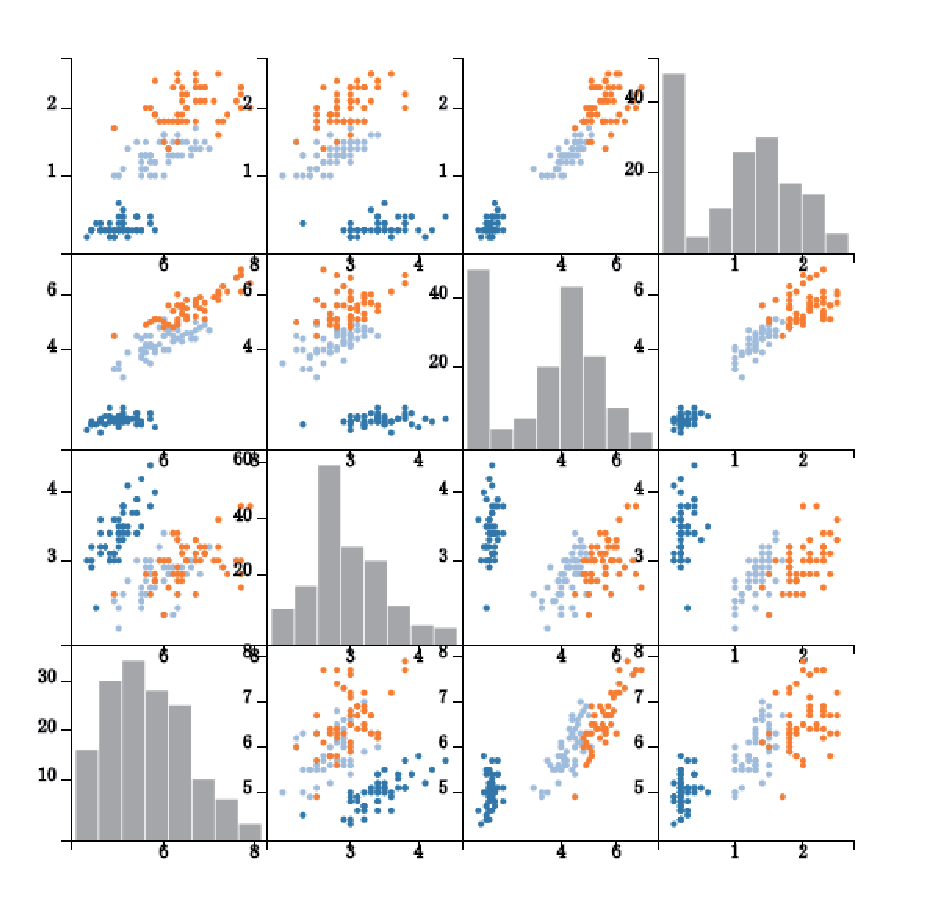
\includegraphics[width=0.99\linewidth]{images/scatterplotmatrix.eps}
% \caption{Designing a scatter-plot matrix visualization with VisComposer.}
% \label{fg:scatterplotmatrix}
%\end{figure}

\subsection{Tag Cloud}
VisComposer supports the visualization of a collection of words with the tag cloud  techniques. Figure~\ref{teaser} (e) is an example of the tag cloud based on the~\emph{Countries and Dependencies by Population Dataset}\footnote{Countries and dependencies by population, \url{http://en.wikipedia.org/wiki/List\_of\_countries\_and\_dependencies\_by\_population}. (last accessed: 2015.03.31)}. Here, the font size of the words is  proportional to the  word frequency, which can be achieved by binding the word frequency with the color with a linear mapping in the Transformation module. Additionally, a visualization shader is created based on a randomized greedy strategy to layout the words. The font color can be interactively bound to a categorical dimension of the dataset.


\subsection{Squarified Treemaps}
 % hand-coded programmable module
 % scenegraph and the content of programmable module needed
VisComposer is capable of crafting recursive layouts, like the treemap. A treemap consist of a recursive drawing layout which is difficult to design with a static scenegraph structure. To handle the recursion, a custom composition can be created by using a visualization shader in the transformation module. Figure~\ref{teaser} (f) shows the visualization of the~\emph{Public Company Bankruptcy Cases Dataset}~\footnote{Public Company Bankruptcy Cases Opened and Monitored for Fiscal Year 2009, \url{http://catalog.data.gov/dataset}. (last accessed: 2015.03.31)}, and the associated scenegraph and workflow. It should be noted that the squarified layout is implemented without using any existing JavaScript visualization libraries. To support the color assignment on the rectangles, a color mapping transformation is created afterwards.
%  of JSON data with hierarchical structure
% \begin{figure}
%  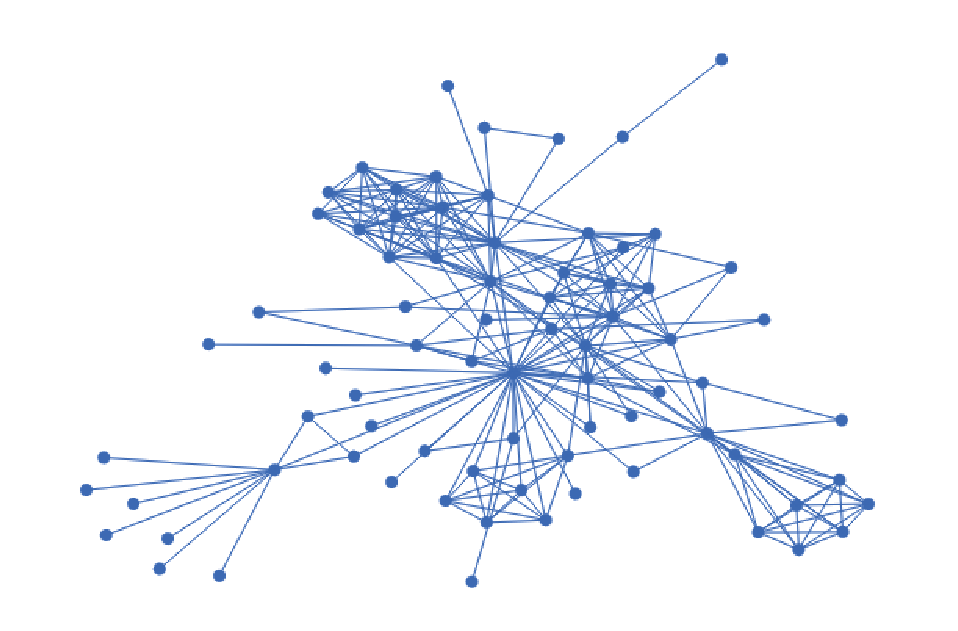
\includegraphics[width=0.99\linewidth]{images/force-directed.eps}
%   \caption{Designing a squarfied treemap with VisComposer. : (a) The result of treemap layout; (b) the scenegraph; (c) the workflow; and (d) the programmable transformation.}
%   \label{fg:treemap}
% \end{figure}



%To bind the line width of links to a feature of the data, a non-linear visual mapping transformation is created with a modifier of user-defined statement.

%where \texttt{d3.layout.force} is utilized

%\begin{figure}
% 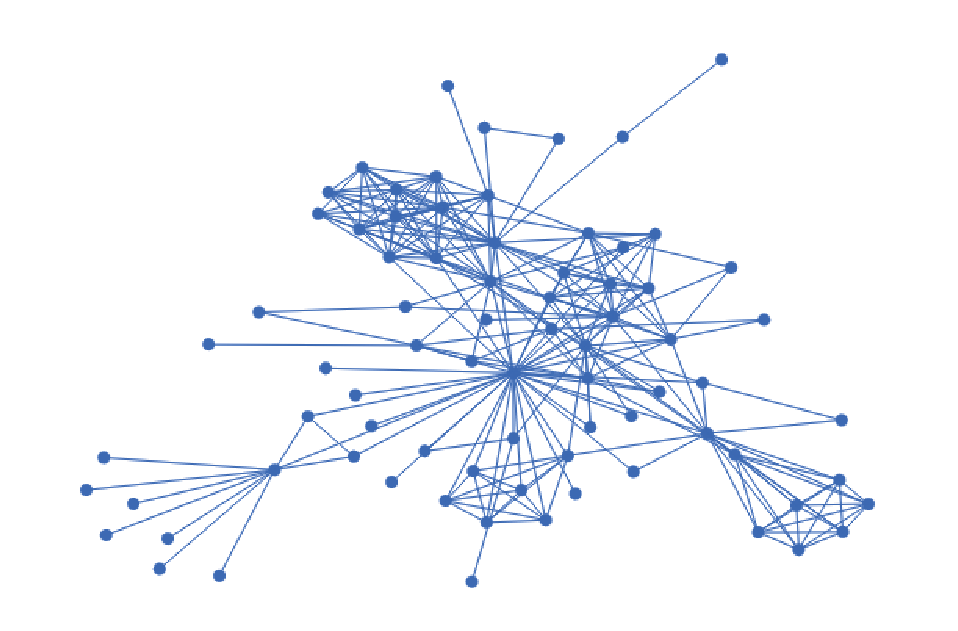
\includegraphics[width=0.99\linewidth]{images/force-directed.eps}
%   \caption{Designing a force-directed graph with VisComposer. The link width is used to encode a data dimension.}
%   \label{fg:forcelayout}
% \end{figure}


%
% \begin{figure}
%  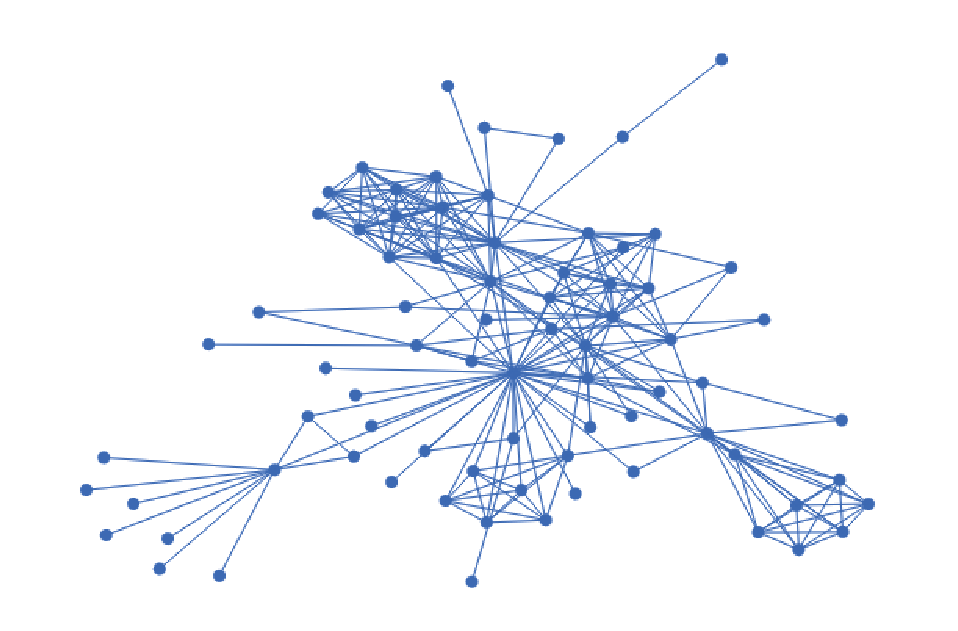
\includegraphics[width=0.99\linewidth]{images/force-directed.eps}
%   \caption{Case 4: bubble plot.}
%   \label{fg:bubble_plot}
% \end{figure}






%Its composition operator is an implementation of a randomized greedy algorithm coded in Custom Module, which can fullfill all kind of composition operators using Javascript or d3.js. VisComposer also make some special tag cloud, for example, tags of random font-family, thanks to its powerful flexibility.

 %Its composition operator is an implementation of a randomized greedy algorithm coded in Custom Module, which can fullfill all kind of composition operators using Javascript or d3.js. VisComposer also make some special tag cloud, for example, tags of random font-family, thanks to its powerful flexibility.

% \begin{figure}
%  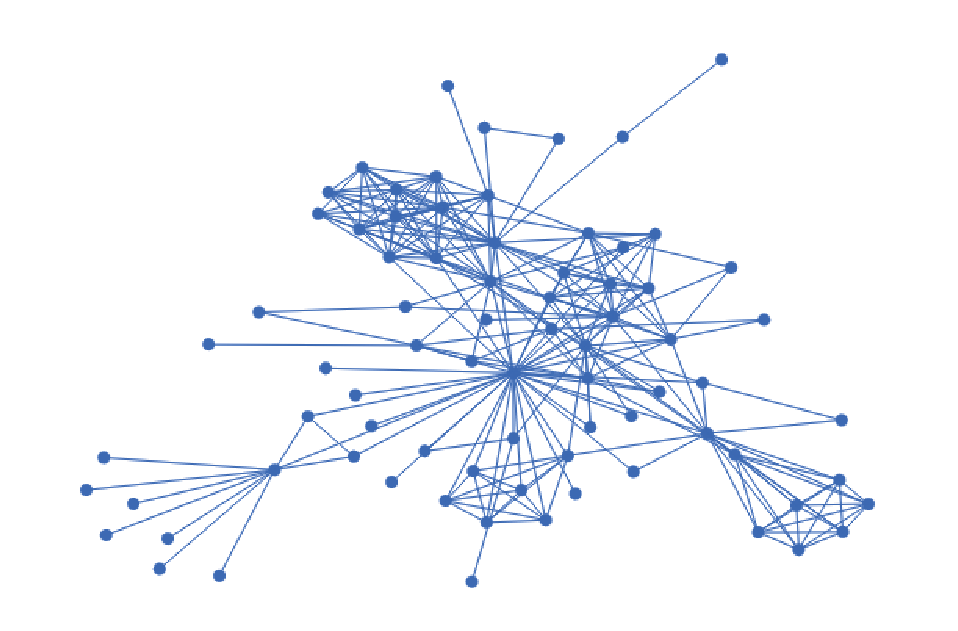
\includegraphics[width=0.99\linewidth]{images/force-directed.eps}
%   \caption{Designing the tag cloud visualization with VisComposer.}
%   \label{fg:tagcloud}
% \end{figure}

% \subsection{Time-series Data}
%
% \subsection{Spatio-temporal Data}

%
%
%\begin{figure} [!htb]
%\centering
%\begin{tabular}{cc}
%\includegraphics[width=0.45\columnwidth]{Figures/PicSummary_1.eps} &
%\includegraphics[width=0.45\columnwidth]{Figures/PicSummary_2.eps} \\
%(a) & (b) \\
%\includegraphics[width=0.45\columnwidth]{Figures/DocSegmentation.eps} &
%\includegraphics[width=0.45\columnwidth]{Figures/SemanticReoccur.eps} \\
%(c) & (d) \\
%\end{tabular}
%\caption{Visualizing a section of ``My life". (a-b) Two pictorial summarizations of two different topics; (c) A piece of \emph{hphc} that
% shows the process of Clinton's second contest for the Governor of Arkansas in 1982.
%  (d) A repetitive appearance in the $\emph{hphc}$ reveals the entire procedure of the President election preparation of Bill Clinton in 1991.}
%\label{fig:tools}
%\end{figure}
